\subsection{Training and Tuning}\label{sec:training-and-tuning}

Experiments are conducted on shared nodes of the bwHPC cluster, with 10 assigned Intel Xeon Gold 6230 cores at \SI{2.1}{\GHz}, an NVIDIA V100 \SI{32}{\giga\byte}, and \SI{92.160}{\giga\byte} random access memory running Red Hat Enterprise Linux release 8.4. For reproducibility, the implementation and experiment tracking are publicly available.\footnote{Code is available at~\url{https://github.com/KarelZe/thesis} Experiments are tracked at \url{https://wandb.ai/fbv/thesis}.}

\subsubsection{Training of Supervised
    Models}\label{sec:training-of-supervised-models}

Our implementation of \glspl{GBRT} is based on CatBoost \autocite[][5--6]{prokhorenkovaCatBoostUnbiasedBoosting2018} because of its efficient implementation on \glspl{GPU} and native support for categorical variables. However, as discussed in \cref{sec:gradient-boosting-procedure}, we expect the chosen library to have minimal impact on performance.

\begin{figure}[ht]
    \centering
    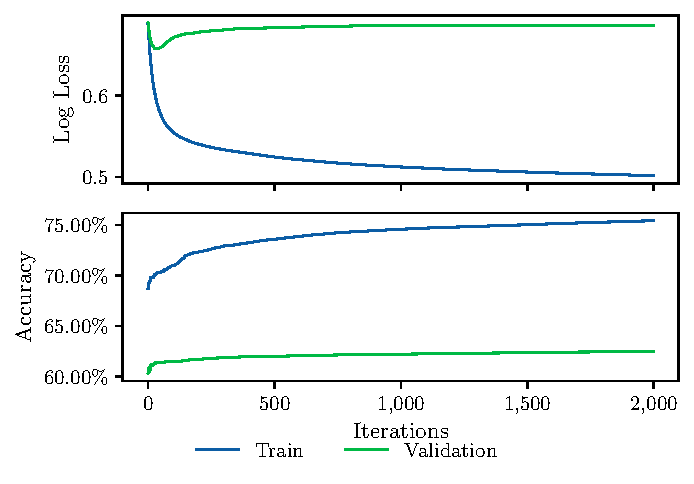
\includegraphics{gbm-train-val-loss-acc.pdf}
    \caption[Training and Validation Accuracy of Gradient-Boosting]{Training and validation accuracy of \gls{GBRT} on \gls{ISE} sample. Metrics are estimated on the classical feature set. One iteration corresponds to an additional regression tree added to the ensemble. Loss is expected to decrease for more complex ensembles and accuracy to increase.}
    \label{fig:gbm-train-val-loss-acc}
\end{figure}

\cref{fig:gbm-train-val-loss-acc} displays the loss and accuracies of the default implementation on the \gls{ISE} training and validation set using classical features. The plots reveal several insights.

Firstly, the model overfits the training data, as evident from the generalisation gap between training and validation accuracies. To improve generalisation performance, we apply regularisation techniques.

Secondly, validation loss spikes for larger ensembles, while validation accuracy continues to improve. This discrepancy suggests that the predicted class's correctness improves, but the ensemble becomes less confident in the correctness of the prediction.

\begin{figure}[ht]
    \centering
    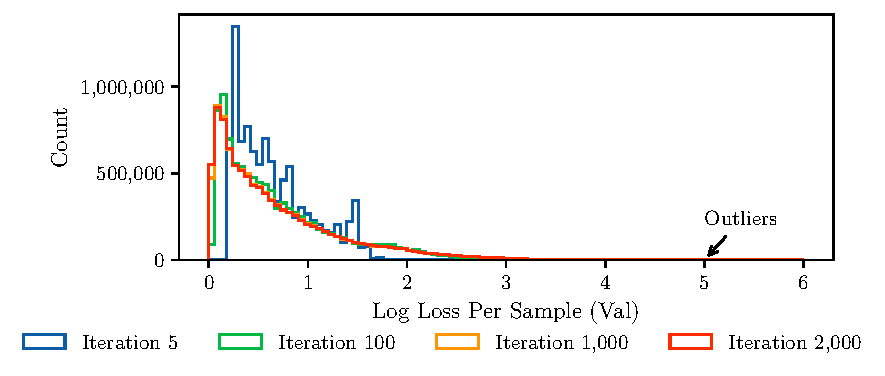
\includegraphics{gbm-loss-distribution.pdf}
    \caption[Sample-Wise Log Loss of Gradient-Boosting]{Sample-wise log loss of \glsentryshort{GBRT} on \glsentryshort{ISE} sample as equi-width histogram. Loss is estimated on the classical feature set. In general, log loss improves for larger ensembles, as indicated by the increased number of samples accumulating around zero but few predictions contribute to the loss unproportionally causing the log loss to stagnate on average.}
    \label{fig:gbm-loss-distribution}
\end{figure}

This behaviour can be explained by the log loss being unbound, where single incorrect predictions can cause the loss to explode. We verify this assumption by plotting the distribution of the sample-wise log loss in \cref{fig:gbm-loss-distribution}. As visible, loss per sample decreases for larger ensembles, at the same time few predictions contribute to the loss unproportionally, causing the average validation loss to stagnate.

\begin{figure}[ht]
    \centering
    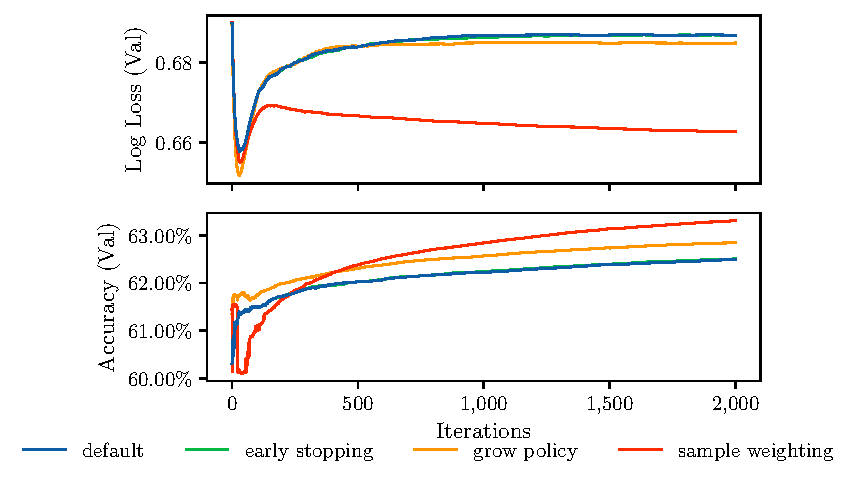
\includegraphics{gbm-optimisations-loss-acc.pdf}
    \caption[Training and Validation Accuracy of \glsentryshort{GBRT} with Optimisations]{Training and validation accuracy of \gls{GBRT} on \gls{ISE} sample with optimisations. Metrics are estimated on the classical feature set. One iteration corresponds to an additional regression tree added to the ensemble. Loss is expected to decrease for more complex ensembles and accuracy to increase.}
    \label{fig:gbm-optimisations-loss-acc}
\end{figure}

We leverage several architectural changes to reduce the loss, further improve performance and mitigate overfitting in gradient boosting, as shown in \cref{fig:gbm-optimisations-loss-acc}, where the effects on validation accuracy and log loss over the default configuration are visualised. Following standard practice, e.g., \textcite{tuningplaybookgithub}, all other parameters are kept at their default values, while a single parameter is varied to derive the plots. Although this approach ignores parameter interactions, it still can guide the optimal training configuration. We train on the ISE training set with classical features and report metrics on the validation set.

\emph{Growth Strategy}

To improve performance, we switch to a leaf-wise growth strategy, following \textcite[][4]{chenXGBoostScalableTree2016}. By default, CatBoost grows oblivious regression trees, which are symmetric and grown level-wise. In this strategy, splits are performed on the same feature and split values across all nodes of a single level, which is computationally efficient but may compromise performance. In contrast, leaf-wise growth selects terminal nodes that provide the largest improvement in the loss, potentially leading to nodes within the same level being split with different features and values, resulting in a closer fit to the data. Leaf-wise growth also aligns with the intuition of split finding from \cref{sec:decision-tree}. This change improves validation accuracy by \SI{0.3461}{\percent} but has little effect on the loss.

\emph{Sample Weighting}

The work of \textcite[][36--38]{grauerOptionTradeClassification2022} suggests a strong temporal shift in the data, with the performance of classical trade classification rules deteriorating over time.  As a result, the predictability of features derived from these rules diminishes over time, and patterns learnt from old observations become less relevant for predicting test samples. To address this, we introduce a sample weighting scheme that assigns higher weights to recent training samples and gradually decays weights over time, which we incorporate into the log loss. Validation and test samples are equally weighted. Sample weighting proves to be essential for achieving high validation performance, and it positively impacts the accuracy and confidence in the prediction mitigating the problem from above.

\emph{Border Count}

In regression trees of gradient-boosting, the split finding is typically approximated with quantization, whereby all numeric features are first discretised into a fixed number of buckets through histogram building, and splits are evaluated at the border of the buckets \autocite[][2]{keLightGBMHighlyEfficient2017}. To increase the number of split candidates, we raise the border count to \num{254}. Generally, this leads to increased accuracy at the cost of computational efficiency. Yet, in the experiment above, the improvements in validation loss and accuracy are minor compared to the previous modifications.

\emph{Early Stopping and Checkpointing}

To reduce overfitting, we monitor the training and validation accuracies when adding new trees to the ensemble and suspend training once validation accuracy decreases for \num{100} iterations. The ensemble is then cut back to achieve the highest validation accuracy. In the experiment above, early stopping does not apply, as validation accuracy continues to improve for larger ensembles. We employ additional measures to address overfitting but treat them as a tunable hyperparameter, with further details provided in \cref{sec:hyperparameter-tuning}.

We incorporate these ideas to leverage the improvements for our large-scale studies.

\textbf{Transformer}

As derived in \cref{sec:supervised-approaches}, we rely on the FT-Transformer of \textcite[][4--5]{gorishniyRevisitingDeepLearning2021} as our second model. The training of Transformers has been found non-trivial and requires a carefully designed training setup of model, optimizer, and learning rate schedule \autocite[][1]{liuUnderstandingDifficultyTraining2020}. We investigate minor modifications to the default FT-Transformer to stabilise training and improve overall performance. The default FT-Transformer trained for 10 epochs on \gls{ISE} dataset with classical features and loss and accuracy is visualised in \cref{fig:fttransformer-optimisations-loss-acc}.\footnote{Default configuration documented in \textcite[][18]{gorishniyRevisitingDeepLearning2021}.}

The convergence behaviour of our model is similar to that of gradient boosting. Equally, a significant generalisation gap exists between the training and validation loss. Particularly concerning, the training loss decreases sharply, while the validation loss spuriously improves over its initial estimate. Despite this, validation accuracy improves throughout the entire training cycle. We reason that the network learns to correctly classify trades, indicated by the improved accuracy, but only attains low-confident correct predictions or confident but erroneous predictions which both contribute to a large validation loss. The shape of the flat validation loss and the decreasing training loss suggest that the training set may not be representative of trades in the validation set. This has broader implications on the classifiability of option trades using decision rules from classical trade classification rules for more recent observations. We explore this phenomenon thoroughly as part of our result discussion.

\begin{figure}[!ht]
    \centering
    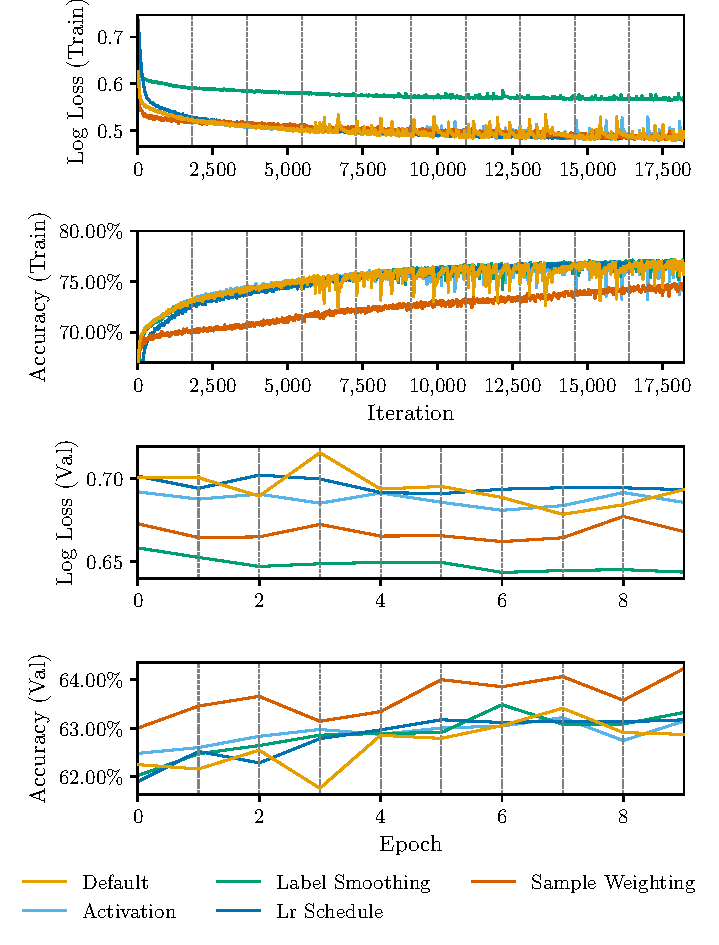
\includegraphics{fttransformer-optimisations-loss-acc.pdf}
    \caption[Training and Validation Accuracy of FT-Transformer with Optimisations]{Training and validation accuracy of FT-Transformer on \gls{ISE} sample with optimisations. Metrics are estimated on the classical feature set. One iteration corresponds to one gradient update. The end of each epoch is marked with a dashed bar. Loss is expected to decrease throughout training and accuracy to increase.}
    \label{fig:fttransformer-optimisations-loss-acc}
\end{figure}

\textbf{Solutions For FT-Transformer}

\emph{Activation Function}

Motivated by previous research, we experiment with replacing the $\operatorname{ReLU}$ activation with the $\operatorname{GELU}$ activation function \autocite[][2]{hendrycksGaussianErrorLinear2020} in the classification head and the gated variant $\operatorname{ReGLU}$ with the gated variant $\operatorname{GEGLU}$ \autocite[][2]{shazeerGLUVariantsImprove2020} in the \gls{FFN}. As visualised in \cref{fig:fttransformer-optimisations-loss-acc}, no advantage in terms of validation accuracy or loss is evident.

\emph{Sample Weighting}

We apply the concept of sample weighting from \gls{GBRT} to Transformers. Specifically, we scale the contribution of individual training samples to the loss using a sample weight, which penalises the model for misclassifying recent observations. This method is crucial for achieving low validation loss and high validation accuracies, as visible in \cref{fig:fttransformer-optimisations-loss-acc}. The significantly lower training accuracy implies, that patterns from latter observations do not universally transfer to previous observations. At this time, it remains unclear what is causing the data drift within the training set.

\clearpage

\emph{Label Smoothing}

A major problem in classification with neural networks is, that the network becomes over-confident in predicting training samples but performs poorly on unseen data. In \cref{fig:fttransformer-optimisations-loss-acc} the effect is evident, as the increased confidence in the prediction on the training set does not transfer to the validation set. To regularise the network, we experiment with label smoothing \autocite[][2823]{szegedyRethinkingInceptionArchitecture2016} by training on soft labels with an uncertainty constant of $\epsilon$. Instead of assigning hard class probabilities of 0 or 1, we assume that true labels in the training set are correct with $1-\epsilon$ probability and incorrect otherwise. For $\epsilon=\num{0.1}$, a trade with the true label $-1$ is assumed to be \SI{90}{\percent} seller-initiated and \SI{10}{\percent} buyer-initiated. While we observe that label smoothing improves the validation loss and reduces the generalisation gap, we find that it has a negligible effect on validation accuracy and therefore abandon this approach.

\emph{Learning Rate Schedule}

When training Transformers, the learning rate is often adjusted throughout the training process. \textcite[][7]{vaswaniAttentionAllYou2017} use a learning rate warm-up period, whereby the learning rate is linearly increased in the early stages of training, followed by decay using an inverse square root learning rate schedule. The warm-up phase is thought to stabilise gradients as weight updates are considerably smaller. According to the research of \textcite[][3--4]{xiongLayerNormalizationTransformer2020}, learning rate warm-up is crucial for training post-norm Transformers, but optional for pre-norm Transformers like the FT-Transformer. Nevertheless, we experiment with the effect of learning rate warm-up in our setting and combine a linear warm-up for two epochs with subsequent cosine decay, as visualised in \cref{fig:lr-lin-warmup-cosine-decay}.

\begin{figure}[!ht]
    \centering
    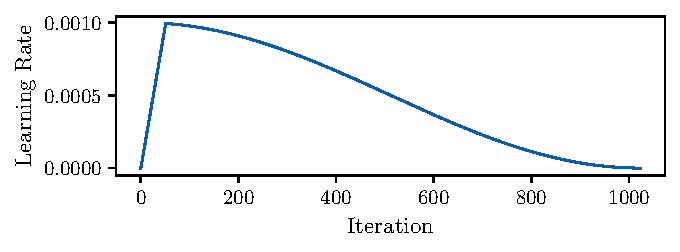
\includegraphics{lr-lin-warmup-cosine-decay.pdf}
    \caption[Linear Learning Rate Warm-Up With Cosine Decay]{Linear learning rate warm-up with cosine decay. Warm-up is performed for the first \SI{5}{\percent} of iterations. In the example, the maximum learning rate is \num{1e-3}.}
    \label{fig:lr-lin-warmup-cosine-decay}
\end{figure}

The scheduled learning rate has soothing effects on the training loss and accuracy estimates, as evident in \cref{fig:fttransformer-optimisations-loss-acc}. Therefore, we adopt a training setup with a learning rate schedule, despite the potential negative effects on training time. The learning rate itself is tuned as part of \cref{sec:hyperparameter-tuning}.


\emph{Batch Size}

% 20 epochs (\num{36460} / \num{145840} iterations) 
We use a fixed batch size of \num{8192} samples for the feature set classical / classical-size and \num{2048} for the feature set option, which is the largest possible size on our \gls{GPU}. Training is performed for \num{20} epochs at maximum. All samples within the training and validation set are shuffled randomly to promote convergence. Although a smaller batch size could enhance the generalisation capabilities of the model, as found in \textcite[][3]{keskarLargeBatchTrainingDeep2017}, we train on the largest number of trades per iteration, to optimise throughput. Additional regularisation is added to the model, but treated as a tunable hyperparameter.

\emph{Early Stopping and Checkpointing}

Similar to the \gls{GBRT}, we halt training prematurely based on a consecutive decrease in validation accuracy. We set the patience to \num{10} epochs and restore the best model in terms of validation accuracy from the checkpoint. Checkpoints are saved at the end of each epoch. In the experiment above, early stopping does not apply.

\emph{Optimizer}

In line with \textcite[][6]{gorishniyRevisitingDeepLearning2021}, we train the models using the AdamW optimizer \autocite[][2--3]{loshchilovDecoupledWeightDecay2019} with the standard hyperparameters~\footnote{Parameters $\beta_{1}=0.9, \beta_{2}=0.999$, and $\epsilon = \num{1e-8}$}. The weight decay coefficient in AdamW determining the degree of regularisation is tuned in \cref{sec:hyperparameter-tuning}. Weight decay is selectively applied and excludes embeddings, LayerNorm, and biases.

In summary, we extend the training setup of \textcite[][6]{gorishniyRevisitingDeepLearning2021} with a sample weighting scheme and learning rate schedule aimed at boosting performance and training stability.

\textbf{Solutions For Classical Rules}

Classical trade classification rules serve as a benchmark in our work. We implement them as a classifier that combines arbitrary trade classification rules through stacking, as covered in \cref{sec:semi-supervised-approaches}.

In cases where classification is not feasible due to missing data or the rules' definition itself, we resort to a random classification, which achieves an average accuracy of \SI{50}{\percent}. The approach is adopted from \textcite[][887]{savickasInferringDirectionOption2003}.

\subsubsection{Training of Semi-supervised
    Models}\label{sec:training-of-semi-supervised-models}

This section discusses the extensions necessary to train the semi-supervised variants of \glspl{GBRT} and the FT-Transformer.

\textbf{Gradient Boosting With Self-Training}

To incorporate unlabelled trades into the training procedure, we combine gradient boosting with a self-training classifier, as derived in \cref{sec:extensions-to-gradient-boosted-trees}. We repeat self-training for 2 iterations and require the predicted class probability to exceed $\tau=0.9$. As the entire ensemble is rebuilt three times, the relatively low number of iterations and high confidence threshold, strike a balance between computational requirements and the need for high-quality predictions. The base classifier is otherwise identical to supervised gradient boosting from \cref{sec:training-of-supervised-models}.

\textbf{Transformer with Pre-Training}

The FT-Transformer is trained in two stages. First, we train for \num{20} epochs on unlabelled \gls{ISE} trades using the \gls{RTD} head, followed by \num{20} epochs of fine-tuning on labelled \gls{ISE} training data with the binary classification head.

During pre-training and fine-tuning, early stopping is applied based on the value of the objective on the validation set, using patience of \num{10}. This particular setup is adopted from \textcite[][15]{rubachevRevisitingPretrainingObjectives2022} for being compute-efficient and offering competitive performance. The hidden dimension of the classification head is set to \num{512}. Based on \textcite[][3]{clarkElectraPretrainingText2020} \SI{15}{\percent} of all tokens are replaced. 

Since the unlabelled sample includes various types of trades that may not be comparable to the labelled sample, we update all layers during fine-tuning. Empirically, finetuning the entire model is among the most successful methods for large-scale Transformers, as results from \textcite[][104--105]{raeScalingLanguageModels2022} indicate.

Following \textcite[][4]{rubachevRevisitingPretrainingObjectives2022}, the learning rate and weight decay are shared between the pre-training and fine-tuning stages. Given the nature of pre-training, all other hyperparameters related to the model are identical.

\subsubsection{Hyperparameter Tuning}\label{sec:hyperparameter-tuning}

All of our machine-learning models feature a set of tunable hyperparameters. The results of previous studies, exemplary the one of \textcite[][5]{grinsztajnWhyTreebasedModels2022}, emphasise the need for tuning routines, as the test performance of the FT-Transformer and \glspl{GBRT} largely fluctuates with the hyperparameter configuration. For a fair comparison, we employ an exhaustive hyperparameter search, to find a suitable hyperparameter configuration for each of our models.

Classical rules have no hyperparameters per se, but the best hybrid rules can be attained through hyperparameter search.

\textbf{Bayesian Search}

We perform a novel Bayesian search to suggest and tune the hyperparameters automatically. In Bayesian search, a prior belief for all possible objective functions is formulated from the parameter intervals, which is then gradually refined by updating the Bayesian posterior with data from previous trials thereby approximating the likely objective function \autocite[][2]{shahriariTakingHumanOut2016}. Compared to brute-force approaches, such as grid search, unpromising search regions are omitted, resulting in more promising trials.

While different algorithmic implementations exist for Bayesian optimisation, we choose the \emph{Optuna} library by \textcite[][1--10]{akibaOptunaNextgenerationHyperparameter2019}, which implements the tree parzen estimator algorithm and is capable of handling both continuous and categorical hyperparameters.\footnote{Implementation of the tree-parzen estimator searches the first 10 trials randomly before the completed trials affect the sampling.} We maximise the accuracy of the validation set, which is also our decisive metric for evaluation (cp. \cref{sec:evaluation-metric}), and run $\num{50}$ trials per feature set for the \gls{GBRT} and $\num{10}$ trials for the FT-Transformer. The best combination of each is tested out-of-sample in \cref{sec:results}.

\textbf{Gradient Boosting}

Our search space is reported in \cref{tab:hyperparameter-space-gbm}, which is aligned with the recommendations in \textcites[][20]{prokhorenkovaCatBoostUnbiasedBoosting2018}[][18]{gorishniyRevisitingDeepLearning2021}[][4]{rubachevRevisitingPretrainingObjectives2022} with minor deviations.

\begin{table}[!h]
    \centering
    \sisetup{table-number-alignment=left}
    \caption[Hyperparameter Search Space of Gradient Boosting]{Hyperparameter search space of gradient boosting.}
    \label{tab:hyperparameter-space-gbm}
    \begin{tabular}{@{}ll@{}}
        \toprule
        Hyperparameter               & Distribution                                  \\ \midrule
        Depth                        & $\operatorname{UniformInt}[1,12]$             \\
        Learning rate $\eta$         & $\operatorname{LogUniform}[0.001, 0.125]$     \\
        $\ell_2$ Leaf Regularisation & $\operatorname{UniformInt}[2, 30]$            \\
        Random Strength              & $\operatorname{LogUniform}[\num{1e-9}, 10.0]$ \\
        Bagging Temperature          & $\operatorname{Uniform}[0.0, 1.0]$            \\ \bottomrule
    \end{tabular}
\end{table}

As documented in \cref{tab:hyperparameter-space-gbm}, we tune five hyperparameters for gradient boosting. The first is the depth, which determines the number of levels in each tree. Other than \textcite[][]{gorishniyRevisitingDeepLearning2021}, we increase the upper bound to twelve to allow for more complex ensemble members. Acknowledging the research of \textcite[][14]{friedmanGreedyFunctionApproximation2001} that the learning rate \eta~and the size of the ensemble have a strong interdependence, we only tune the learning rate and stop extending the ensemble based on the early stopping criterion. Random strength, bagging temperature, and $\ell_2$ leaf regularisation are measures to counter overfitting. Specifically, random strength controls the degree of Gaussian noise added to the scores of split candidates to introduce randomness in the selected splits. In a similar vein, the algorithm introduces randomness on the sample level through Bayesian bootstrap. The hyperparameter controls the distribution used for sampling, and implicitly the aggressiveness of bagging. Finally, $\ell_2$ leaf regularisation adds a penalty term to the terminal leaf's estimates. The hyperparameter controls the degree of regularisation.

\cref{fig:ise-gbm-hyperparam-classical} visualises the hyperparameter search space of the \gls{GBRT} on the \gls{ISE} dataset with classical features, from which we can derive several observations. First, hyperparameter tuning has a significant impact on the prediction, as the validation accuracy varies between \SI{58.429}{\percent} and \SI{64.378}{\percent} for different trials. Second, the best hyperparameter combination, marked with \bestcircle, lies off-the-borders surrounded by other promising trials, indicated by the contours, from which we can conclude, that the found solution is a stable and reasonable choice for further analysis.

\begin{figure}[!h]
    \subfloat[Hyperparameter Search Space of \gls{GBRT} With Feature Set Classical\label{fig:ise-gbm-hyperparam-classical}]{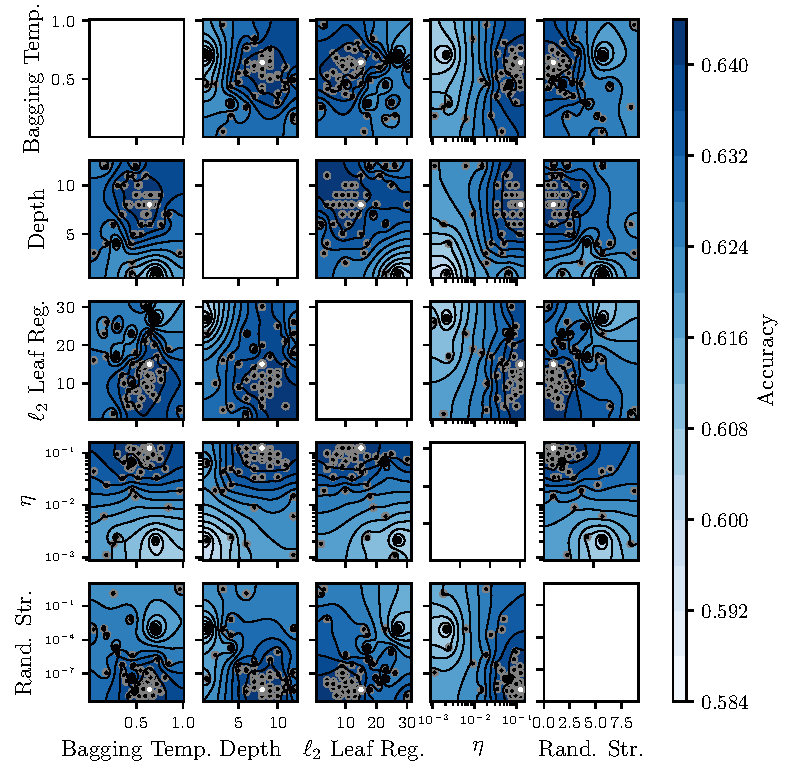
\includegraphics[width=0.6\textwidth]{1gzk7msy-hyperparam-search-space.pdf}}
    \vfill
    \subfloat[Hyperparameter Search Space of \gls{GBRT} With Feature Set Size\label{fig:ise-gbm-hyperparam-classical-size}]{\addtocounter{subfigure}{1}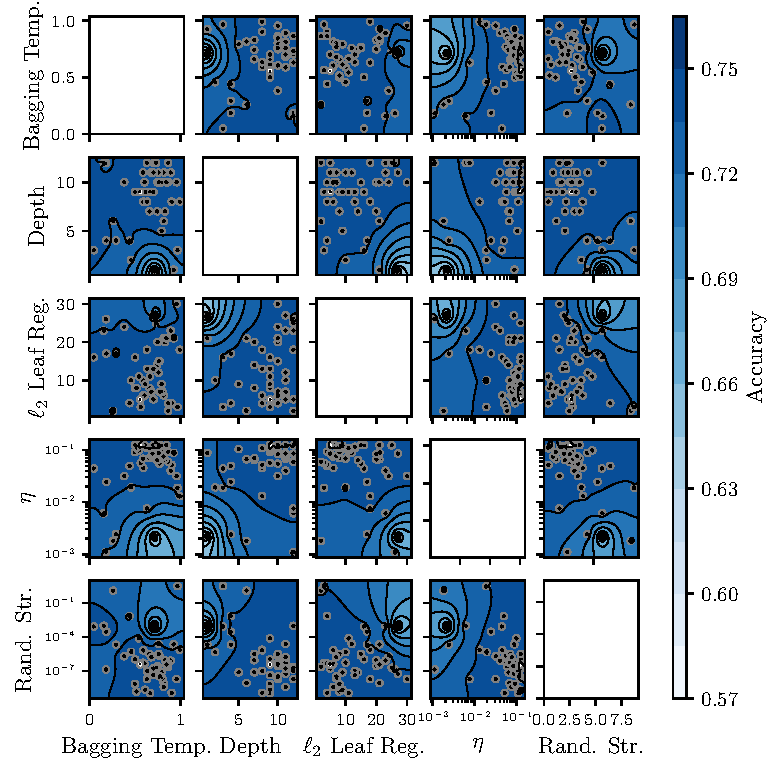
\includegraphics[width=0.6\textwidth]{3vntumoi-hyperparam-search-space.pdf}}
\end{figure}
\clearpage
\begin{figure}[!ht]
    \addtocounter{figure}{-1}
    \subfloat[Hyperparameter Search Space of \gls{GBRT} With Feature Set Option\label{fig:ise-gbm-hyperparam-ml}]{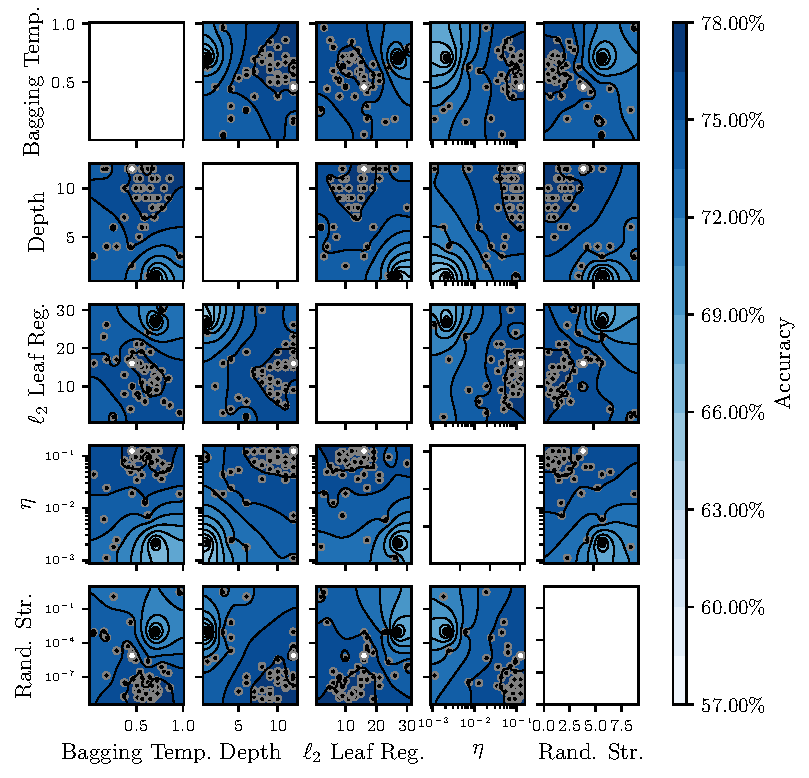
\includegraphics[width=0.6\textwidth]{2t5zo50f-hyperparam-search-space.pdf}}
    \caption[Hyperparameter Search Space of Gradient-Boosting]{Hyperparameter Search Space of \gls{GBRT} on \gls{ISE} Validation Set}
    \label{fig:ise-gbm-hyperparam}
\end{figure}

In \cref{fig:ise-gbm-hyperparam-classical-size} we repeat the analysis for \gls{GBRT} trained on classical-size features. The loss surface is smooth with large connected regions. As the best solution achieving \SI{75.03504680858162}{\percent} accuracy lies within a splayed region of dense sampling, it is a good choice for further analysis. Consistent with the loss surface of \cref{fig:ise-gbm-hyperparam-classical}, the trees are grown to the maximum depth and a high learning rate, indicating the need for complex ensemble members highly corrective to previous predictions. Part of this could be due to the low signal-to-noise ratio in financial data.

The loss surface of the \gls{GBRT} trained on the feature set including option features is the least fragmented. While the validation accuracy of the best combinations improves significantly to \SI{76.99459643967347}{\percent}, worst trials even underperform these of smaller feature sets. Based on this observation we conjecture, that more data does not per se improve the model and that models require a thoughtful tuning procedure. By this means, our conclusion contradicts the one of \textcite[][14]{ronenMachineLearningTrade2022}, who find no advantage in tuning tree-based ensembles for trade classification. Results are tabulated in \cref{tab:solutions-gbm}.

\begin{table}[!h]
    \centering
    \sisetup{table-format=3.2, table-number-alignment=right}
    \caption[Search Solutions of Gradient Boosting]{Search solutions of gradient boosting. The three right columns document the best combination in terms of validation accuracy per feature set. We perform \num{50} trials each.}
    \label{tab:solutions-gbm}
    \begin{tabular}{@{}llSSS@{}}
        \toprule
        Hyperparameter               & Distribution                                  & {\glsentryshort{FS} Classical} & {\glsentryshort{FS} Size} & {\glsentryshort{FS} Option} \\ \midrule
        Depth                        & $\operatorname{UniformInt}[1,12]$             & 8                              & 9                         & 12                          \\
        Learning rate $\eta$         & $\operatorname{LogUniform}[0.001, 0.125]$     & 0.12484221864046671            & 0.12347889459796775       & 0.12471458170177774         \\
        $\ell_2$ Leaf Regularisation & $\operatorname{UniformInt}[2, 30]$            & 15                             & 5                         & 16                          \\
        Random Strength              & $\operatorname{LogUniform}[\num{1e-9}, 10.0]$ & \num{4e-9}                     & \num{4e-7}                & \num{8e-6}                  \\
        Bagging Temperature          & $\operatorname{Uniform}[0.0, 1.0]$            & 0.6419530220498153             & 0.5574912093427532        & 0.45578836944233            \\ \midrule
        Validation Accuracy in \%    &                                               & 64.37816236230594              & 75.03504680858162         & 76.99459643967347           \\ \bottomrule
    \end{tabular}
\end{table}

\textbf{Gradient Boosting With Self-Training}

The search space for the semi-supervised variant is identical to the supervised gradient boosting. To conserve space, we only report the tabulated results in \cref{tab:solutions-GBRT-self-training}. Visualisations of the hyperparameter search space are available online.\footnote{See \url{https://wandb.ai/fbv/thesis/runs/37lymmzc} for \gls{FS} classical, \url{https://wandb.ai/fbv/thesis/runs/324v3uv5} for \gls{FS} size, and \url{https://wandb.ai/fbv/thesis/runs/t55nd8r0} for \gls{FS} option.}

\begin{table}[!h]
    \centering
    \sisetup{table-format=3.2, table-number-alignment=right}
    \caption[Search Solutions of Gradient Boosting With Self-Training]{Search solutions of gradient boosting with self-training. The three right columns document the best combination in terms of validation accuracy per feature set. We perform \num{50} trials each. Arrows indicate the change compared to the supervised variant.}
    \label{tab:solutions-GBRT-self-training}
    \begin{tabular}{@{}llSSS@{}}
        \toprule
        Hyperparameter               & Distribution                                  & {\glsentryshort{FS} Classical}         & {\glsentryshort{FS} Size}              & {\glsentryshort{FS} Option}            \\ \midrule
        Depth                        & $\operatorname{UniformInt}[1,12]$             & 9                                      & 10                                     & 9                                      \\
        Learning rate $\eta$         & $\operatorname{LogUniform}[0.001, 0.125]$     & 0.12337960608926582                    & 0.1248422186404667                     & 0.12347504812996231                    \\
        $\ell_2$ Leaf Regularisation & $\operatorname{UniformInt}[2, 30]$            & 12                                     & 9                                      & 13                                     \\
        Random Strength              & $\operatorname{LogUniform}[\num{1e-9}, 10.0]$ & \num{2e-8}                             & \num{5e-8}                             & \num{5e-8}                             \\
        Bagging Temperature          & $\operatorname{Uniform}[0.0, 1.0]$            & 0.34010535578784745                    & 0.5214954412829511                     & 0.4666577105566224                     \\ \midrule
        \multicolumn{2}{l}{Validation Accuracy in \%}                                               & {$\textcolor{viz-red}{\downarrow} \num{64.29671279599335}$} & {$\textcolor{viz-red}{\downarrow} \num{74.83010065958079}$} & {$\textcolor{viz-red}{\downarrow} \num{76.41433947686962}$} \\ \bottomrule
    \end{tabular}
\end{table}

Matching the supervised results, semi-supervised ensembles exhaust the maximum tree depth and combine trees with a coarse learning rate. By parameter importance, both are most influential on the final result. Again, this is an indication that the trade data is not easily separable, requiring multiple features and splits. The found hyperparameters for $\ell_2$ leaf regularisation, random strength and bagging are balanced. Overall, the best validation accuracies are slightly inferior to the supervised variant.

\clearpage

\textbf{Transformer}

The search space for the FT-Transformer is identical to \textcite[][18]{gorishniyRevisitingDeepLearning2021} (variant (b)) with minor deviations and reported in \cref{tab:hyperparameter-space-2}.

\begin{table}[!h]
    \centering
    \sisetup{table-text-alignment=right}
    \caption[Hyperparameter Search Space of FT-Transformer]{Hyperparameter search space of FT-Transformer.}
    \label{tab:hyperparameter-space-2}
    \begin{tabular}{@{}ll@{}}
        \toprule
        Hyperparameter         & Distribution                                        \\ \midrule
        Layers $L$             & $\operatorname{UniformInt}[1,6]$                    \\
        Attention dropout      & $\operatorname{Uniform}[0, 0.5]$                    \\
        \gls{FFN} dropout      & $\operatorname{Uniform}[0, 0.5]$                    \\
        Learning rate $\eta$   & $\operatorname{LogUniform}[\num{3e-5}, \num{3e-4}]$ \\
        weight decay $\lambda$ & $\operatorname{LogUniform}[\num{1e-6}, \num{1e-3}]$ \\ \bottomrule
    \end{tabular}
\end{table}

We vary the layer count and the embedding dimension, which directly affect the capacity of the network. Layers refer to the number of Transformer blocks in the encoder stack. The dimension of numerical and continuous embeddings $d_e$ is at \num{256} at maximum, which is half the dimension used in the author's work. We make this sacrifice, due to being computation-bound by the size of the dataset. Dropout \autocite[][1930]{srivastavaDropoutSimpleWay} in the attention module and the \gls{FFN} is used to prevent overfitting the training data. As discussed in \cref{sec:training-of-supervised-models}, we treat the weight decay term in the weight update rule of the AdamW optimizer as a hyperparameter, with larger values for \lambda~enforcing a stronger shrinkage of weights and thereby reducing overfitting.

Due to the pseudo-random sampling during the first trials of Bayesian search combined with the reduced number of trials for the Transformer studies, the tested hyperparameter combinations are identical for all feature sets, as visible in \cref{fig:ise-transformer-hyperparam}.

\begin{figure}[!h]
    \subfloat[Hyperparameter Search Space of FT-Transformer With Feature Set Classical\label{fig:ise-transformer-hyperparam-classical}]{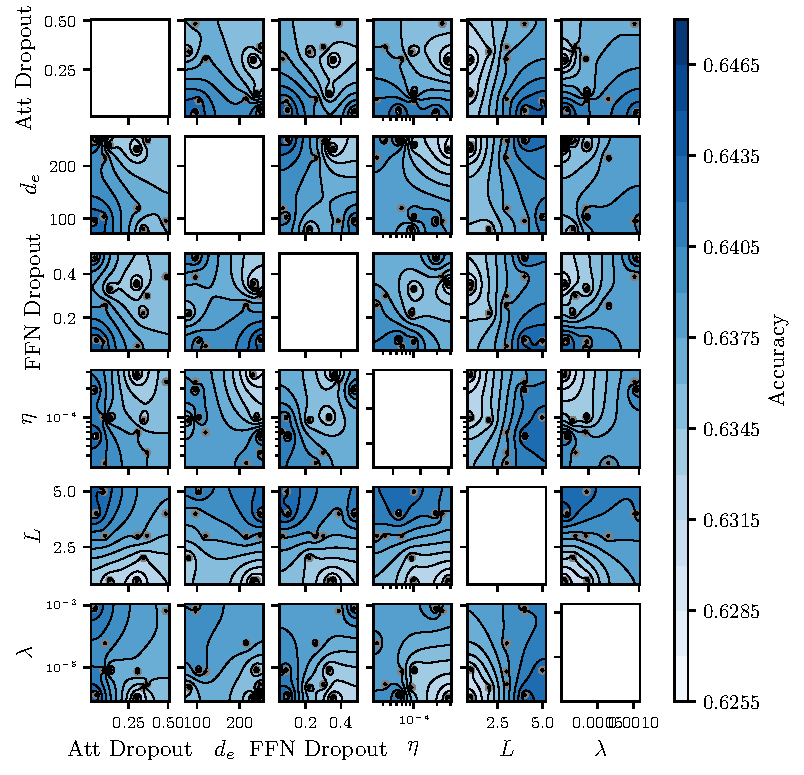
\includegraphics[width=0.6\linewidth]{3jpe46s1-hyperparam-search-space.pdf}}
    \vfill
    \subfloat[Hyperparameter Search Space of FT-Transformer With Feature Set Size\label{fig:ise-transformer-hyperparam-classical-size}]{\addtocounter{subfigure}{1}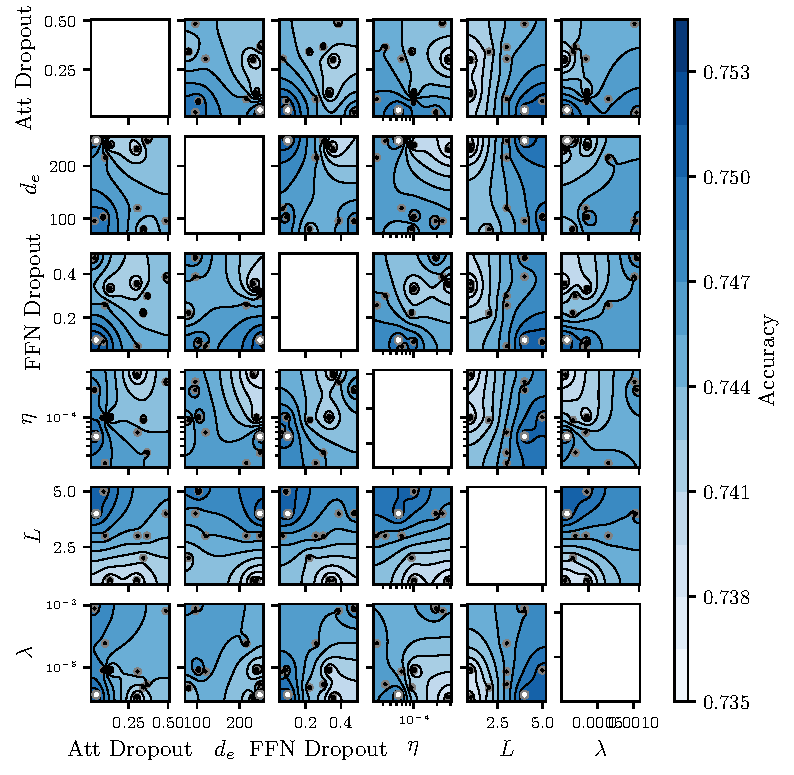
\includegraphics[width=0.6\linewidth]{1qx3ul4j-hyperparam-search-space.pdf}}
\end{figure}
\clearpage
\begin{figure}[!ht]
    \addtocounter{figure}{-1}
    \subfloat[Hyperparameter Search Space of \gls{GBRT} With Feature Set Option\label{fig:ise-transformer-hyperparam-ml}]{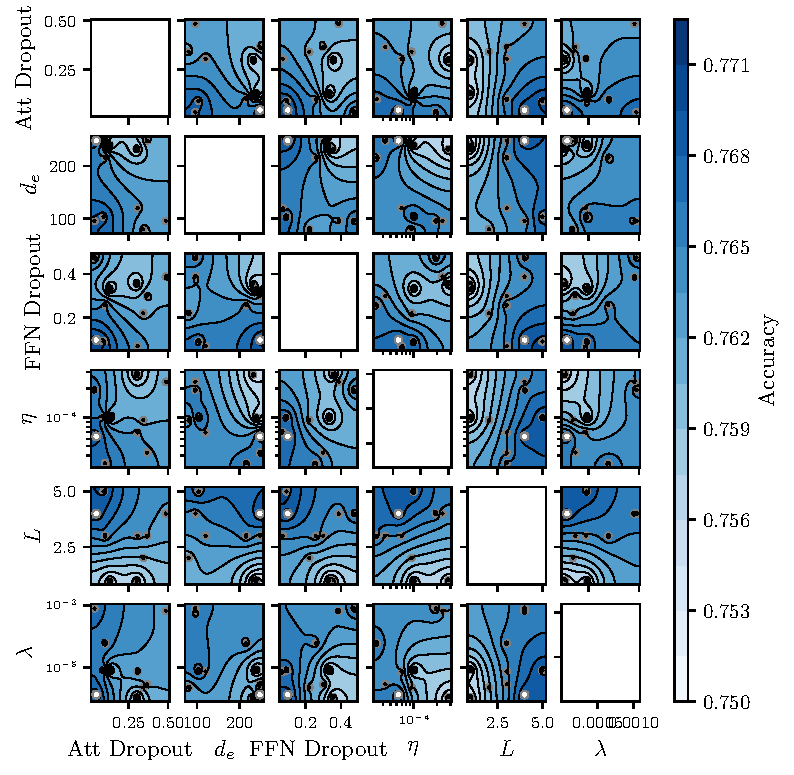
\includegraphics[width=0.6\linewidth]{2h81aiow-hyperparam-search-space.pdf}}
    \caption[Hyperparameter Search Space of FT-Transformer]{Hyperparameter Search Space of FT-Transformer on \gls{ISE} Validation Set}
    \label{fig:ise-transformer-hyperparam}
\end{figure}

With the smaller number of trials, the search space is less densely populated. Despite the decreased coverage, for the searched combinations the impact of hyperparameter tuning is less pronounced than for the \gls{GBRT}. As such, accuracies for \cref{fig:ise-transformer-hyperparam} fluctuate between \SI{62.55}{\percent} and \SI{64.65}{\percent}. This translates to other feature sets. Unaffected, the validation accuracies are higher than for gradient boosting.

The best combination is identical for all feature sets. The embedding dimension is at \num{248}, which is almost maxed out and the model uses four Transformer blocks. Thus, it has a medium capacity with \num{1985649} to \num{4252369} parameters, depending on the feature set. From all hyperparameters, the number of layers is most impactful on the final accuracy. While the use of dropout and weight decay for regularisation is minimal and marginally affects the validation performance. The large token dimensionality and mid-layer count could be an indication, that few attention heads are enough to extract patterns, but the learned patterns are relatively complex. The search results are compiled in \cref{tab:solutions-transformer}.

\begin{table}[!h]
    \centering
    \sisetup{table-format=3.2, table-number-alignment=right}
    \caption[Search Solutions of FT-Transformer]{Search solutions of FT-Transformer. The three right columns document the best combination in terms of validation accuracy per feature set. We perform \num{10} trials each. A discussion of these results is provided below.}
    \label{tab:solutions-transformer}
    \begin{tabular}{@{}llSSS@{}}
        \toprule
        Hyperparameter                       & Distribution                                        & {\glsentryshort{FS} Classical} & {\glsentryshort{FS} Size} & {\glsentryshort{FS} Option} \\ \midrule
        Layers $L$                           & $\operatorname{UniformInt}[1,6]$                    & 4                              & 4                         & 4                           \\
        Embedding dimension $d_{\mathrm{e}}$ & $\operatorname{UniformInt}[64, 256]$                & 248                            & 248                       & 248                         \\
        Attention dropout                    & $\operatorname{Uniform}[0, 0.5]$                    & 0.04424625102595975            & 0.04424625102595975       & 0.04424625102595975         \\
        \gls{FFN} dropout                    & $\operatorname{Uniform}[0, 0.5]$                    & 0.0979914312095726             & 0.0979914312095726        & 0.0979914312095726          \\
        Learning rate $\eta$                 & $\operatorname{LogUniform}[\num{3e-5}, \num{3e-4}]$ & \num{1e-6}                     & \num{1e-6}                & \num{1e-6}                  \\
        Weight decay $\lambda$               & $\operatorname{LogUniform}[\num{1e-6}, \num{1e-3}]$ & \num{6e-5}                     & \num{6e-5}                & \num{6e-5}                  \\ \midrule
        \multicolumn{2}{l}{Validation Accuracy in \%}                                                     & 64.69                          & 75.42                     & 77.17                       \\ \bottomrule
    \end{tabular}
\end{table}

\vskip 1.3in

\textbf{Transformer With Pre-Training}

The hyperparameter search space for Transformers with a pre-training objective is identical to that shown in \cref{tab:hyperparameter-space-2}. As evident from \cref{tab:solutions-transformer-pretraining}, the found solutions are identical to these of the FT-Transformer without pre-training and identical for all three feature sets. During pre-training, we can detect if an token is replaced with \SI{94.06319856643677}{\percent} to \SI{95.89540958404541}{\percent} accuracy.\footnote{Na\"ive prediction yields \SI{85}{\percent} accuracy given the chosen replacement rate.} Validation accuracy after finetuning improves for all models over Transformers without pretraining. As the search space is identically sampled for both variants we can directly attribute the improvements of \SI{0.28}{\percent} to \SI{0.72}{\percent} in validation accuracy to pre-training on unlabelled trades. \todo{Optionally, add a visualisation of pre-training on validation performance (loss + accuracy). Due to reproducible sampling, the effect on validation performance can directly be inferred.} Visualisations of the hyperparameter search spaces are available online.\footnote{See \url{https://wandb.ai/fbv/thesis/runs/12isqh2m} for \gls{FS} classical, for \url{https://wandb.ai/fbv/thesis/runs/2hv1nayy} for \gls{FS} size, and \url{https://wandb.ai/fbv/thesis/runs/3jbqpp4r} for \gls{FS} option for details.}


\begin{table}[!h]
    \centering
    \sisetup{table-format=3.2, table-number-alignment=right}
    \caption[Search Solutions of FT-Transformer With Pre-training]{Search solutions of FT-Transformer with pretraining. The three right columns document the best combination in terms of validation accuracy per feature set. We perform \num{10} trials each. Arrows indicate the change compared to the supervised variant.}
    \label{tab:solutions-transformer-pretraining}
    \begin{tabular}{@{}llSSS@{}}
        \toprule
        Hyperparameter                       & Distribution                                        & {\glsentryshort{FS} Classical}       & {\glsentryshort{FS} Size}            & {\glsentryshort{FS} Option} \\ \midrule
        Layers $L$                           & $\operatorname{UniformInt}[1,6]$                    & 4                                    & 4                                    & 4                           \\
        Embedding dimension $d_{\mathrm{e}}$ & $\operatorname{UniformInt}[64, 256]$                & 248                                  & 248                                  & 248                         \\
        Attention dropout                    & $\operatorname{Uniform}[0, 0.5]$                    & 0.04424625102595975                  & 0.04424625102595975                  & 0.04424625102595975         \\
        \gls{FFN} dropout                    & $\operatorname{Uniform}[0, 0.5]$                    & 0.0979914312095726                   & 0.0979914312095726                   & 0.0979914312095726          \\
        Learning rate $\eta$                 & $\operatorname{LogUniform}[\num{3e-5}, \num{3e-4}]$ & \num{1e-6}                           & \num{1e-6}                           & \num{1e-6}                  \\
        Weight decay $\lambda$               & $\operatorname{LogUniform}[\num{1e-6}, \num{1e-3}]$ & \num{6e-5}                           & \num{6e-5}                           & \num{6e-5}                  \\ \midrule
        Validation Accuracy \%               & Pre-Train                                           & {\num{95.89540958404541}}            & {\num{95.64009308815002}}           & {\num{94.06319856643677}}   \\
                                             & Fine-Tune                                           & {$\textcolor{viz-green}{\uparrow}\num{65.13623935106421}$} & {$\textcolor{viz-green}{\uparrow} \num{75.69871634547757}$} & {$\textcolor{viz-green}{\uparrow} \num{77.8904}$}  \\ \bottomrule
    \end{tabular}
\end{table}

\textbf{Classical Rules}

Akin to selecting the machine learning classifiers, we select our classical baselines on the \gls{ISE} validation set. This prevents \gls{overfitting} the test set and maintains consistency between both paradigms. For the same reason, baselines are kept constant in the transfer setting on the \gls{CBOE} sample.

Optimising hybrids of trade classification rules through Bayesian search is experimentally feasible by the stacking paradigm of \cref{sec:rule-based-approaches} and by treating the rules as a tunable hyperparameter. We consider all rules from \cref{sec:rule-based-approaches} learned on adjacent quotes of the exchange and \gls{NBBO} level or adjacent prices at the exchange and inter-exchange level and stack up to six rules. To model simple rules, consisting of a single or few rules, we add an identity mapping, $\operatorname{Id}$, that defers classification to later rules in the stack. A caveat of this approach is that sampled combinations may not be economically meaningful e.g., applying depth rule after tick rule, or not effective e.g., quote rule after tick rule, assuming complete data. Despite being unexplored, a conditional search space or human-in-the-loop sampling could account for this.

After all, we find no outperformance over hybrid rules already reported in the literature, as documented online.\footnote{For \gls{FS} classical our best combination of $\operatorname{quote}_{\mathrm{nbbo}} \to \operatorname{quote}_{\mathrm{ex}} \to \operatorname{rtick}_{\mathrm{all}}$ (simplified) reaches a validation accuracy of \SI{58.93934926393819}{\percent} equalling the solution of \textcite[][12]{grauerOptionTradeClassification2022}. For \gls{FS} size/option the best search solution is $\operatorname{tsize}_{\mathrm{ex}} \to \operatorname{depth}_{\mathrm{ex}} \to \operatorname{quote}_{\mathrm{nbbo}} \to \operatorname{tick}_{\mathrm{all}}$ (simplified) with \SI{69.03521015523933}{\percent} accuracy. The combination of \textcite[][14]{grauerOptionTradeClassification2022} reaches with $\operatorname{tsize}_{\mathrm{ex}} \to \operatorname{quote}_{\mathrm{nbbo}} \to \operatorname{quote}_{\mathrm{ex}} \to \operatorname{depth}_{\mathrm{nbbo}} \to \operatorname{depth}_{\mathrm{ex}} \to \operatorname{rtick}_{\mathrm{all}}$ an accuracy of \SI{69.3726}{\percent}. See \url{https://wandb.ai/fbv/thesis/runs/3f2m9c6i} and \url{https://wandb.ai/fbv/thesis/runs/16d6e4dk} for details. Experiments are run with \num{500} trials each.} Our combinations match or trail the accuracies of rules from \textcite[][12--14]{grauerOptionTradeClassification2022} on the \gls{ISE} validation set. Subsequently, we adopt their combinations as our benchmark, considering them to be the most challenging.

From all candidate algorithms, a combination of quote and tick rules, $\operatorname{quote}_{\mathrm{nbbo}} \to \operatorname{quote}_{\mathrm{ex}} \to \operatorname{rtick}_{\mathrm{all}}$, where the quote rule first applied to the \gls{NBBO} and then to quotes of the \gls{ISE} followed by the reverse tick rule at inter-exchange level, performs best reaching a validation accuracy of \SI{58.76225138074204}{\percent}. The rule can be estimated using features from feature set one, which qualifies it as a benchmark.

For the second feature set involving size-related rules, we consider rules that involve the trade size or depth rule. Consistent with the recommendation of \textcite[][14]{grauerOptionTradeClassification2022}, we find that a deep stack of the $\operatorname{tsize}_{\mathrm{ex}} \to \operatorname{quote}_{\mathrm{nbbo}} \to \operatorname{quote}_{\mathrm{ex}} \to \operatorname{depth}_{\mathrm{nbbo}} \to \operatorname{depth}_{\mathrm{ex}} \to \operatorname{rtick}_{\mathrm{all}}$ achieves the highest validation accuracy. Much of the performance gains are owed to the trade size and depth rules, which reduce the dependence on the reverse tick test as a last resort and provide overrides for trades at the quotes, improving validation accuracy to \SI{69.37267458589436}{\percent}. Due to the extended use of the quoted sizes and trade sizes, it is our benchmark for the second feature set.

In the absence of other baselines, we repeatedly compare against the same method as a baseline for the third feature set, even if it doesn't involve option-specific features.

In the direct comparison between the validation accuracies of classical rules and our classifiers, the validation accuracies of classical rules considerably underperform the learnt classifier. \cref{sec:results} discusses if the results hold for the test sets. But before we do so, we present the metrics used
for evaluation.